%%%%%%%%%%%%%%%%%%%%% chapter.tex %%%%%%%%%%%%%%%%%%%%%%%%%%%%%%%%%
%
% sample chapter
%
% Use this file as a template for your own input.
%
%%%%%%%%%%%%%%%%%%%%%%%% Springer-Verlag %%%%%%%%%%%%%%%%%%%%%%%%%%

\chapter{Distributed File Systems}

\section{Problems and Goals}
When you want to have a file syustem and manage files, you need to consider following problems:
\begin{itemize}
    \item Naming: allow uses to find files with a human-friendly name.
    \item Accessing: create, delete, read, write, append
    \item Physical Allocation
    \item Security and Protection: ensure privacy
    \item Resource Administration: enforce \underline{quotas} and implement priorities.
\end{itemize}

Besides the problems in mind when design a DFS (actually general file system), we have some goals for DFS. \textbf{The big difference isn't what it does but the environment in which it lives.} A distributed file system typically operates in an environment where the data may be spread out across many, many hosts on a network, and the users of the system may be equally distributed.
\begin{itemize}
    \item Coordinate file systems on machines.
    \item Hide the existence of distributed file system from the user.
\end{itemize}

\textbf{Why we need a DFS.} Actually this problem can be generalized into a problem of distributed system. 
\begin{itemize}
    \item More storage
    \item More fault tolerance
    \item Users are distributed who need to access file system from many places.
\end{itemize}

\section{Operations}

\subsection{Unit of Transmission}
There is a lot of data movement across the network, \textbf{how much do we move one time?} There are two intuitive answers to this question: whole files and blocks.
\begin{itemize}
    \item File: Only the users know how to use the data in one file. File systems do not need to get known how a file is organized.
    \item Block: Reduce the payload for one operation. When the first block of the file arrives, the user can start to operate it.
\end{itemize}

\subsection{Implementation Idea}
\subsubsection{Caching}
Cache is the same usage. Cache data and reduce access to the servers.
There are two kinds of caching in distributed systems:
\begin{itemize}
    \item Cache and Validate Approach: ask servers that if the data is newest. This approach is used in \emph{NFS}.
    \item Callback: if servers have some modification for files, they inform the users. This approach is used in \emph{AFS} and \emph{Coda}.
\end{itemize}

\section{Coda}
\subsection{Disconnected Operations: cache and write conflict}
\paragraph{hoard daemon.} keep certain files in the client's cache, requesting them as necessary, just in case the client should later find itself unable to communicate with the server. Cache and validate. This ensure the users get access the data efficiently.
\paragraph{write conflict.} keep a version number. Before a client writes a file to the server, it checks the version of the file on the server. 
\begin{itemize}
    \item If that version number matches the version number of the file that the client read before the write, the client is safe and can send the new version of the file. The server can then increment the version number.
    \item If the version number has increased, the client missed a callback promise. Then users must take care of the conflicts.
\end{itemize}

\subsection{Replication: Volume Storage Group}
This part is discussed in the Replication chapter. There are some topics for this. 

First, \textbf{how it requests a file?}
\begin{enumerate}
    \item It asks all replicas for their version number.
    \item It asks the replica with the greatest version number for the file.
    \item If there is a conflict, the client can direct the servers to update or inform them of the conflict.
\end{enumerate}

Second, \textbf{how it writes a file?}
\begin{enumerate}
    \item The clients sends the file to all servers, along with the original CVV.
    \item Each server increments its entry in the file's CVV and ACKS the client.
    \item The client merges the entries from all the servers and sends the new CVV back to each server.
\end{enumerate}

Third, \textbf{what if partition happens?}
If one or more servers fail, the client cannot contact the servers. The collections of volume servers that the client can communicate with is known as \emph{Available Volume Storage Group}. 

If the network is partitioned, Coda will still work, but generate some conflicts and inconsistency. (As is said in Chapter Replication.)

\textbf{If the partitioned or failed servers become accessible, the files need to be updated.} The client needs to check VVV or CVV for conflicts. If there is a conflict, the client drops all callbacks in the volume, \\ \underline{because the servers should have all the callbacks}.

\subsubsection{Conflicts}
There are several kinds of conflicts appearing in this problem.
\begin{itemize}
    \item read before write. When the client decide to write the updates to servers, it needs to check if the update reads before write. Otherwise, it may miss some callbacks. Situation could be that the client is broken down for a while and misses some callbacks.
    \item server consistency. After the updates written back to servers and the client getting the CVVs from servers, the client may find conflict in the CVVs. Situation could be that there is concurrent operation on the files.
    \item partitioned network recovered. Replication inconsistency conflict, users need to take actions.
\end{itemize}

\subsection{Weakly Connected Mode}
If a client finds itself with a limited connection to the servers, it will pick a server and send the update. This server will propagate the update to other servers.

\section{File System Interface}
There are some file systems that are designed at user level, rather than in the kernel.
\subsection{MogileFS}
\paragraph{Difference}
Consider the file systems where files are not changed by users. Users are only allowed to upload and download the files. 
\paragraph{Method}
There are some key idea behind the implementation:
\begin{itemize}
    \item RAID. Replication.
    \item Namespaces, rather than directory tree. In different applications. they can use a same MogileFS, but they can use different name.
\end{itemize}
Because there is little change happened, locks will be rarely used. It makes a lot of work efficient.

\subsection{HDFS}
\paragraph{Difference}
HDFS supports the computation of Hadoop.
 
\paragraph{Idea}
There are some key idea behind the implementation:
\begin{itemize}
    \item The data needs to be very heavily distributed.
    \item The data needs to be local to each other, so the system requires location-awareness. 
    \item The system needs to be implemented in a portable way at the user-level, to be operated at scale.
\end{itemize}


%%%%%%%%%%%%%%%%%%%%%%%% Springer-Verlag %%%%%%%%%%%%%%%%%%%%%%%%%%

% %
% %
% %\ For figures use
% %
% \begin{figure}
% \centering
% % Use the relevant command for your figure-insertion program
% % to insert the figure file.
% % For example, with the option graphics use
% 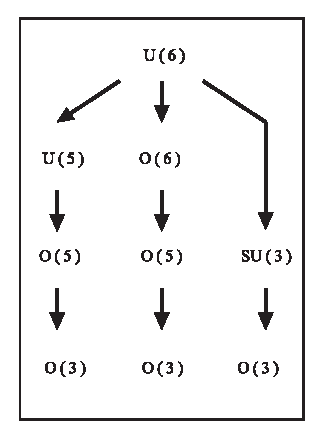
\includegraphics[height=4cm]{figure.eps}
% %
% % If not, use
% %\picplace{5cm}{2cm} % Give the correct figure height and width in cm
% %
% \caption{Please write your figure caption here}
% \label{fig:1}       % Give a unique label
% \end{figure}

% %
% % For tables use
% %
% \begin{table}
% \centering
% \caption{Please write your table caption here}
% \label{tab:1}       % Give a unique label
% %
% % For LaTeX tables use
% %
% \begin{tabular}{lll}
% \hline\noalign{\smallskip}
% first & second & third  \\
% \noalign{\smallskip}\hline\noalign{\smallskip}
% number & number & number \\
% number & number & number \\
% \noalign{\smallskip}\hline
% \end{tabular}
% \end{table}

% % For built-in environments use
% %
% \begin{theorem}
% Theorem text goes here.
% \end{theorem}
% %
% % or
% %
% \begin{lemma}
% Lemma text goes here.
% \end{lemma}
%%%%%%%%%%%%%%%%%%%%%%%% Springer-Verlag %%%%%%%%%%%%%%%%%%%%%%%%%%
